










\subsection{Earth-Sun system}








\subsubsection{Stability}

\begin{figure}[H]
    \centering
    \begin{subfigure}{0.5\textwidth}
        \centering
        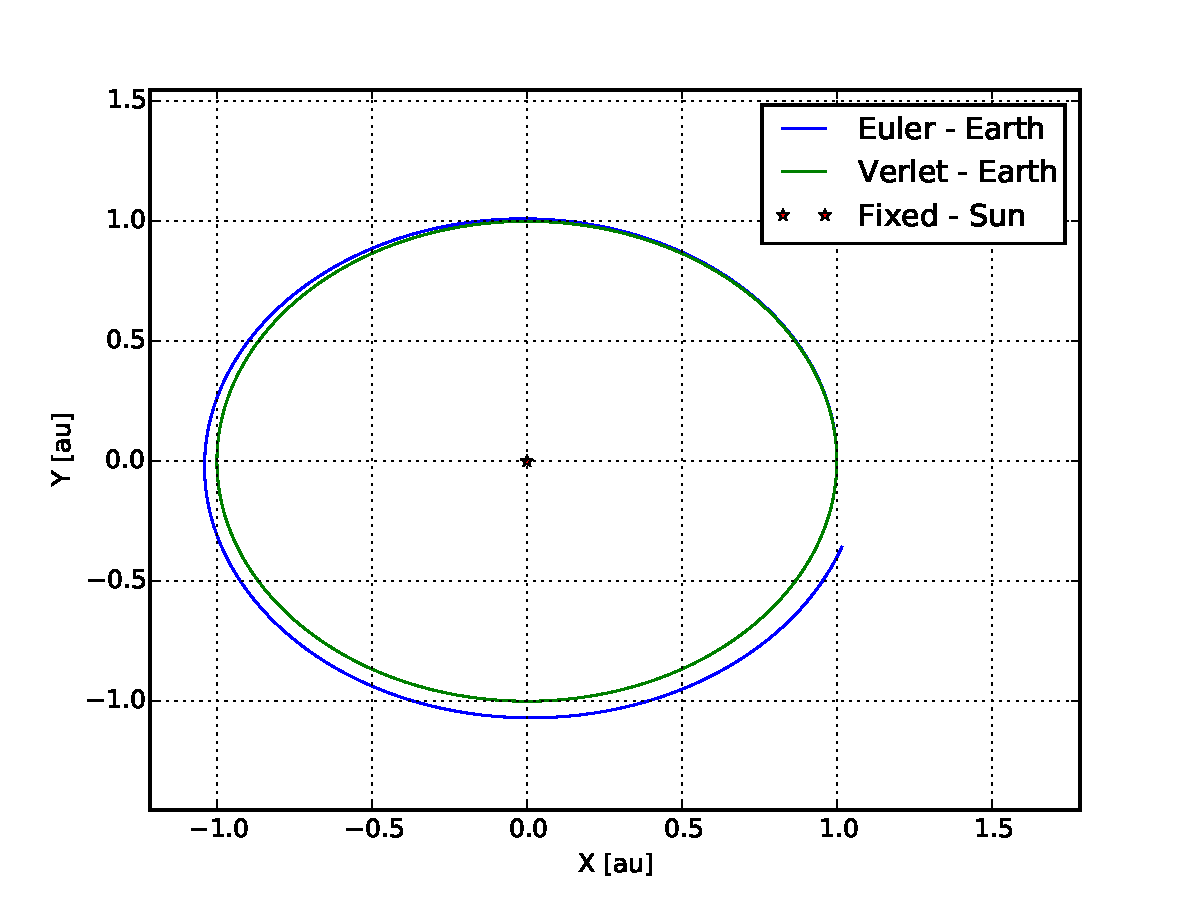
\includegraphics[width=\linewidth]{result/bilder/earth-sun.pdf}
    	\caption{}
    \end{subfigure}%
    ~ 
    \begin{subfigure}{0.5\textwidth}
        \centering
        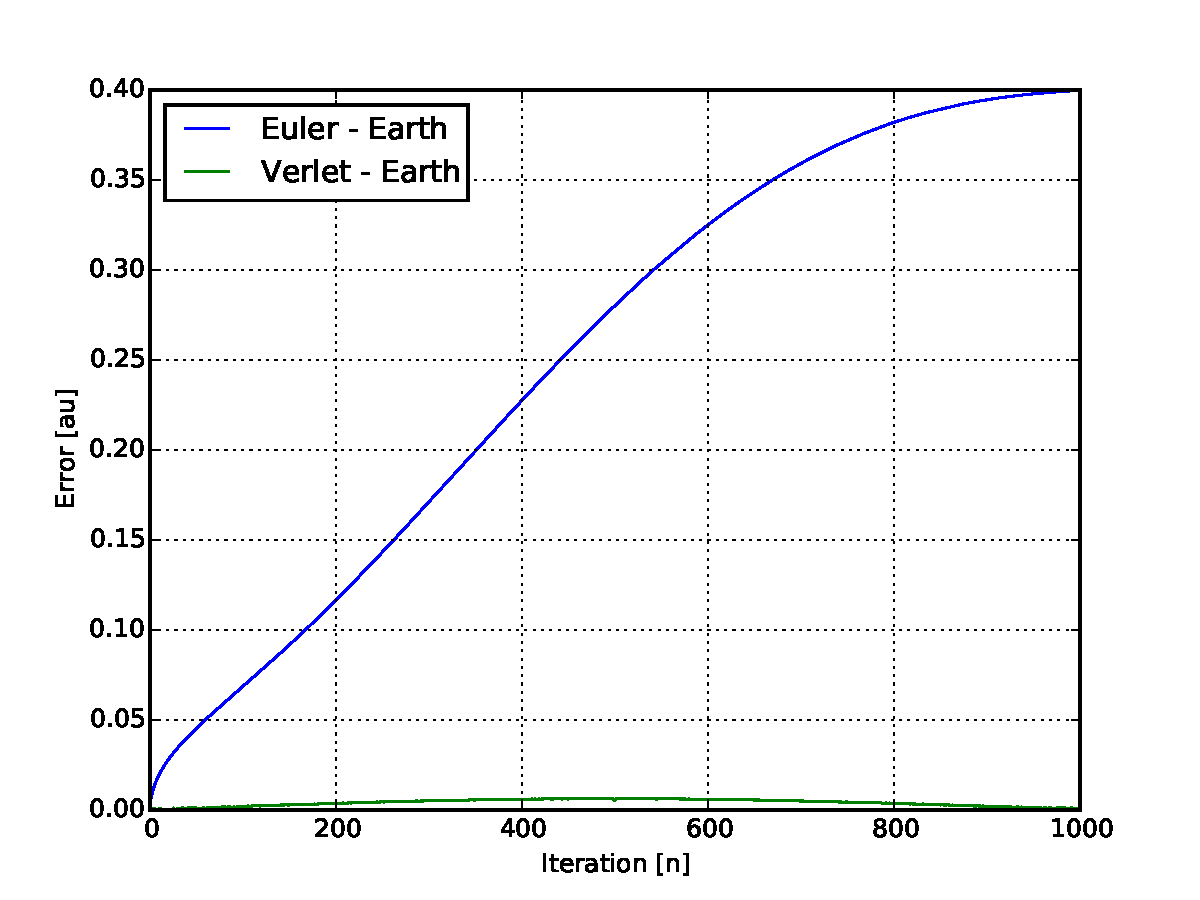
\includegraphics[width=\linewidth]{result/bilder/earth-sun-error.pdf}
        \caption{}
    \end{subfigure}
    \caption{a) show the orbit of earth around the sound. The intial velocity is set to $2\pi$ in y direction and the start position to 1 au in x direction. b) shows how the error behaves. The intial values should give a perfect circular motion. So the error is calculated by $r_i - r_{0}$. It is clear that Verlet-Velocity method is superior. This simulation was with 1000 points with the end time of 1 year. Both simulations was produced by \href{https://github.com/erikfsk/Project-3/blob/master/Project3/3a/plot_earth_sun.py}{\textcolor{blue}{plot\_earth\_sun.py}}}
    \label{fig:earth-sun}
\end{figure}


\todo{REF FLOPS SECTION}
\begin{center}
\label{table:euler-verlet-time}
\captionof{table}{Time table for the different algorithms. The algorithms use nearly the same time. This is not a shocker since the FLOPs are similar. Time grows very linear as expected from FLOPs. Disclaimer: this is only the result from one test, but several was done. Both algorithms were very close and it seem to be random which is fastest.
\\}
\begin{tabular}{|c|c|c|c|c|c|}
    \hline 
    n & Forward-Euler & Verlet-Velocity &  fastest & $\frac{slowest}{fastest}$\\ 
    \hline
    10 & 0.000136 & 0.000148 & Euler &   1.08823529412   \\ 
    \hline 
    100 & 0.000208 & 0.000179 & Verlet &   1.16201117318   \\ 
    \hline 
    1000 & 0.000392 & 0.000389 & Verlet &  1.00771208226   \\ 
    \hline
    10000 & 0.002427 & 0.002426 & Verlet &   1.00041220115  \\ 
    \hline
    100000 & 0.022931 & 0.022293 & Verlet &   1.02861884897   \\ 
    \hline
    1000000 & 0.167022 & 0.175944 & Euler &   1.05341811258  \\ 
    \hline
    10000000 & 1.58721 & 1.52666 & Verlet &   1.03966174525  \\ 
    \hline
    100000000 & 15.1786 & 15.1176 & Verlet &   1.00403503202  \\ 
    \hline
\end{tabular}
\end{center}














\subsubsection{Conserved quantities}

All the figures in this section was made from the data and python script in the directory \href{https://github.com/erikfsk/Project-3/tree/master/Project3/conserved-values}{\textcolor{blue}{conserved-values}}.

\begin{figure}[H]
    \centering
    \begin{subfigure}{0.5\textwidth}
        \centering
        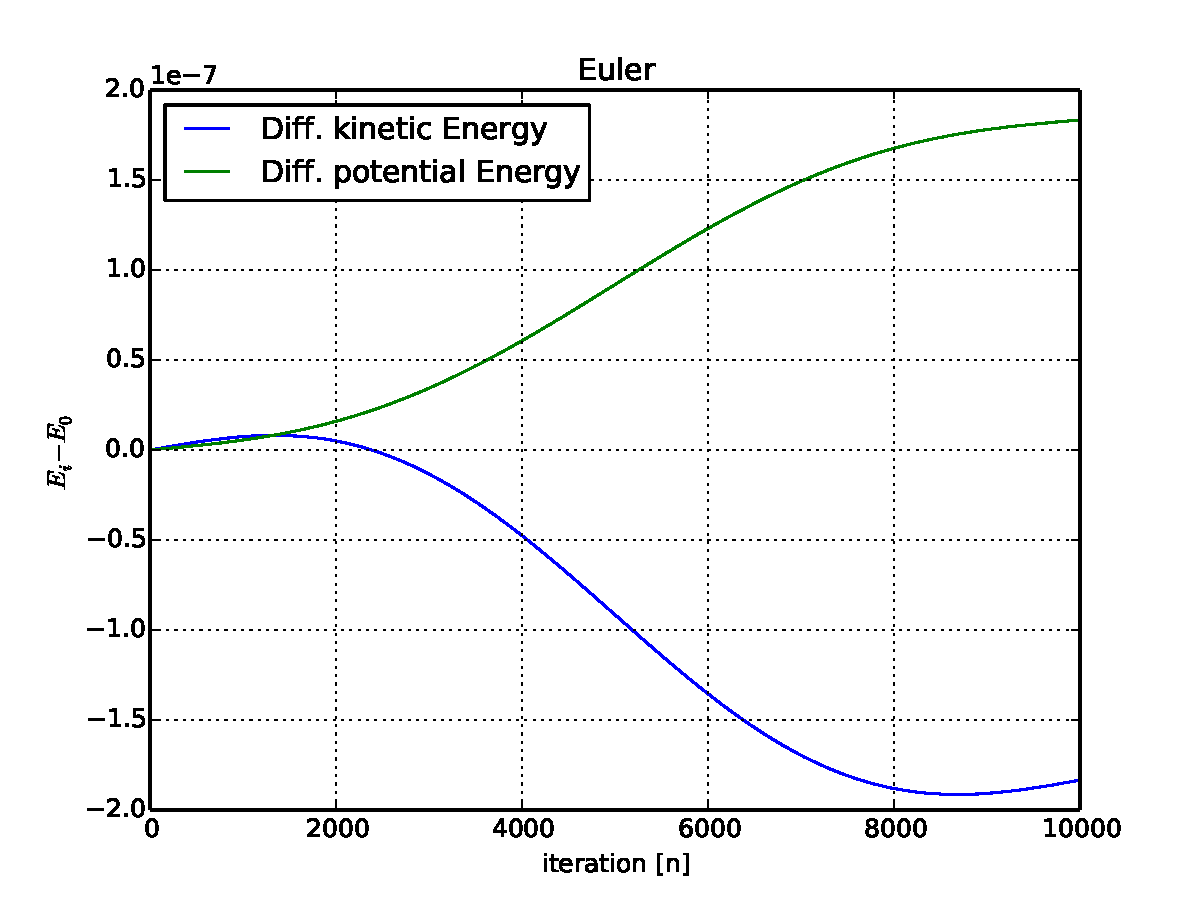
\includegraphics[width=\linewidth]{result/bilder/kin-pot-euler.pdf}
    	\caption{}
    \end{subfigure}%
    ~ 
    \begin{subfigure}{0.5\textwidth}
        \centering
        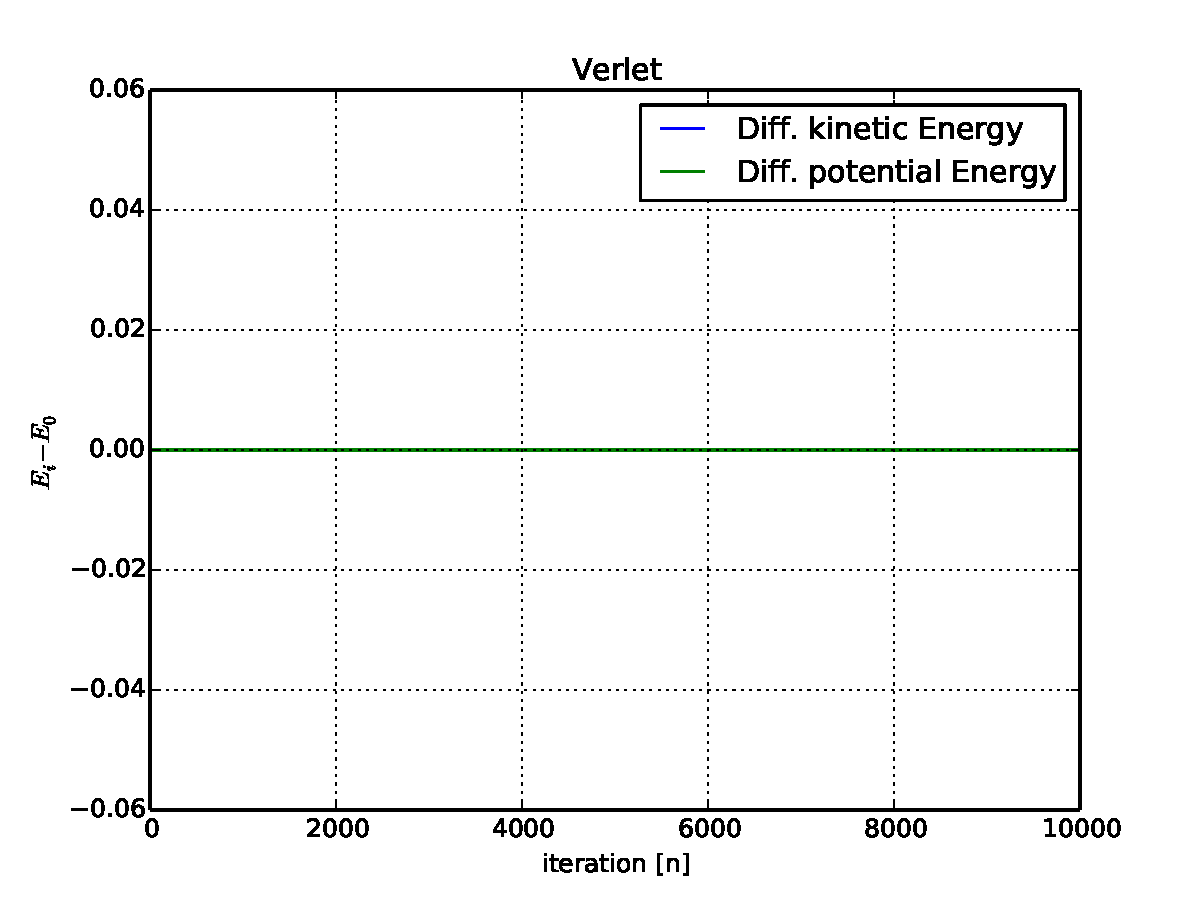
\includegraphics[width=\linewidth]{result/bilder/kin-pot-verlet.pdf}
        \caption{}
    \end{subfigure}
    \caption{Both are figures are graphs of the kinetic energy and potential energy and how it differ from they intial value. a) is the Forward Euler method and b) is the Verlet-Velocity method. As expected the energies are not conserved in the Forward Euler method, but is conserved in the Verlet-Velocity.}
    \label{fig:conserved-energy}
\end{figure}





\begin{figure}[H]
    \centering
    \begin{subfigure}{0.5\textwidth}
        \centering
        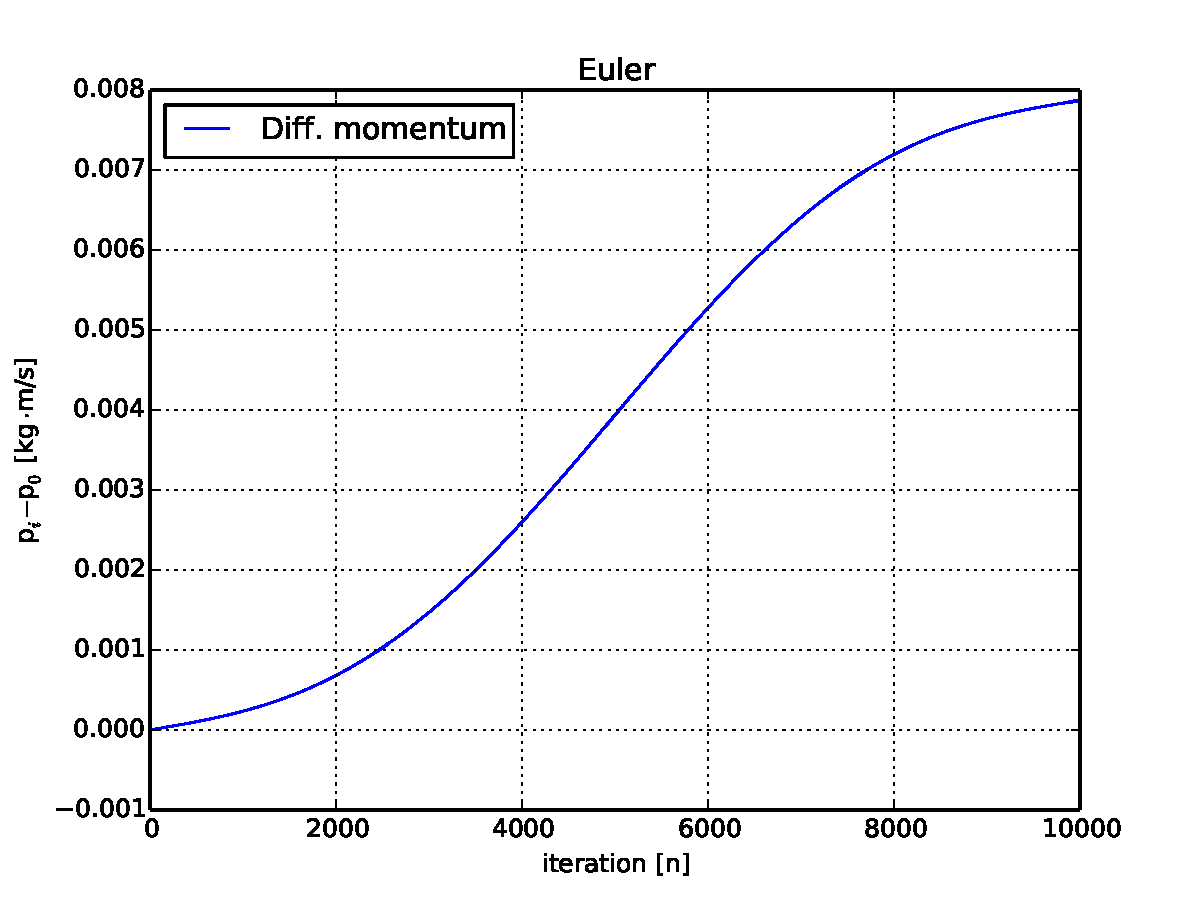
\includegraphics[width=\linewidth]{result/bilder/momentum-euler.pdf}
    	\caption{}
    \end{subfigure}%
    ~ 
    \begin{subfigure}{0.5\textwidth}
        \centering
        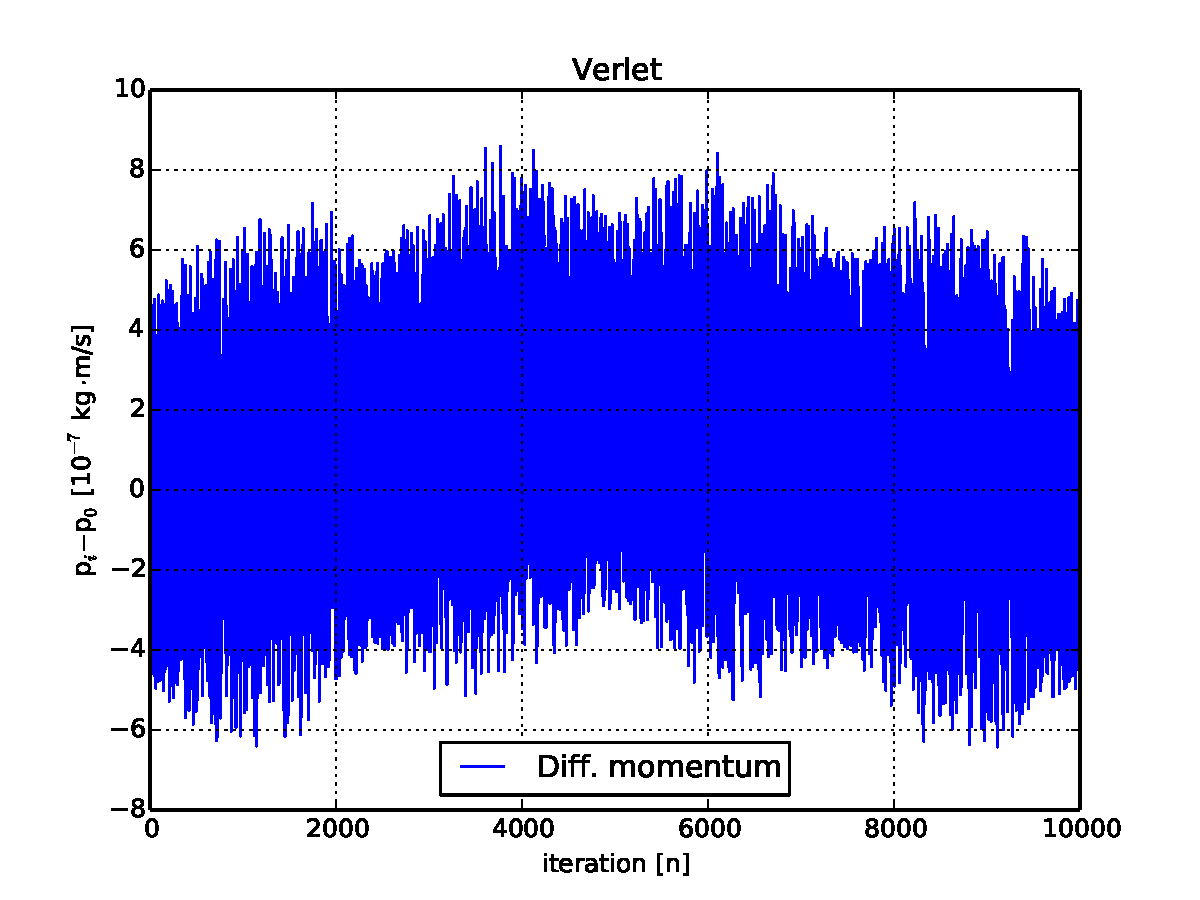
\includegraphics[width=\linewidth]{result/bilder/momentum-verlet.pdf}
        \caption{}
    \end{subfigure}
    \caption{Both are figures are graphs of the momentum and how it differ from they intial value. a) is the Forward Euler method and b) is the Verlet-Velocity method. It should come as no suprise that momentum is not conserved for the Forward Euler method as the kinetic energy was not conserved, as the mass is a constant. Once again the Verlet-velocity method conserve the quantity. 
    }
    \label{fig:conserved-momentum}
\end{figure}





\begin{figure}[H]
    \centering
    \begin{subfigure}{0.5\textwidth}
        \centering
        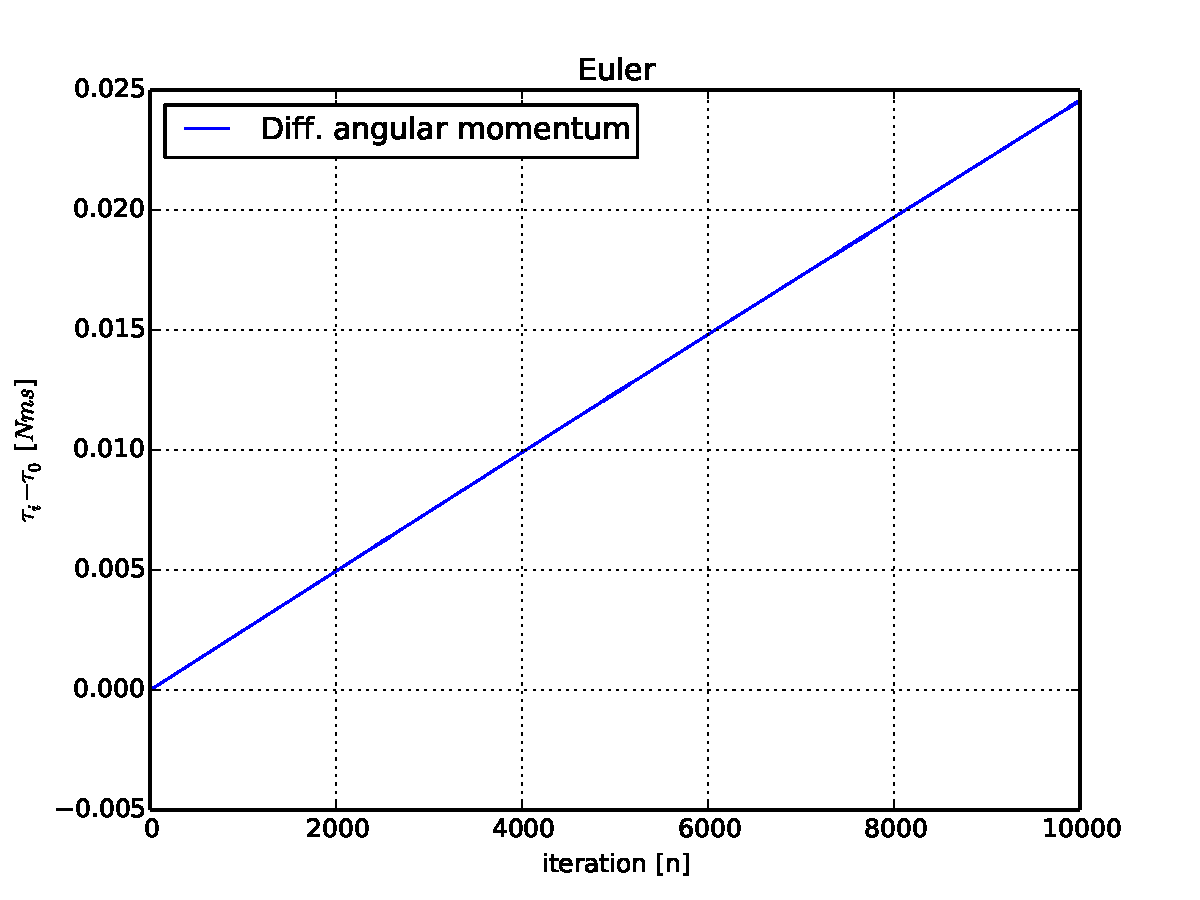
\includegraphics[width=\linewidth]{result/bilder/ang-momentum-euler.pdf}
        \caption{}
    \end{subfigure}%
    ~ 
    \begin{subfigure}{0.5\textwidth}
        \centering
        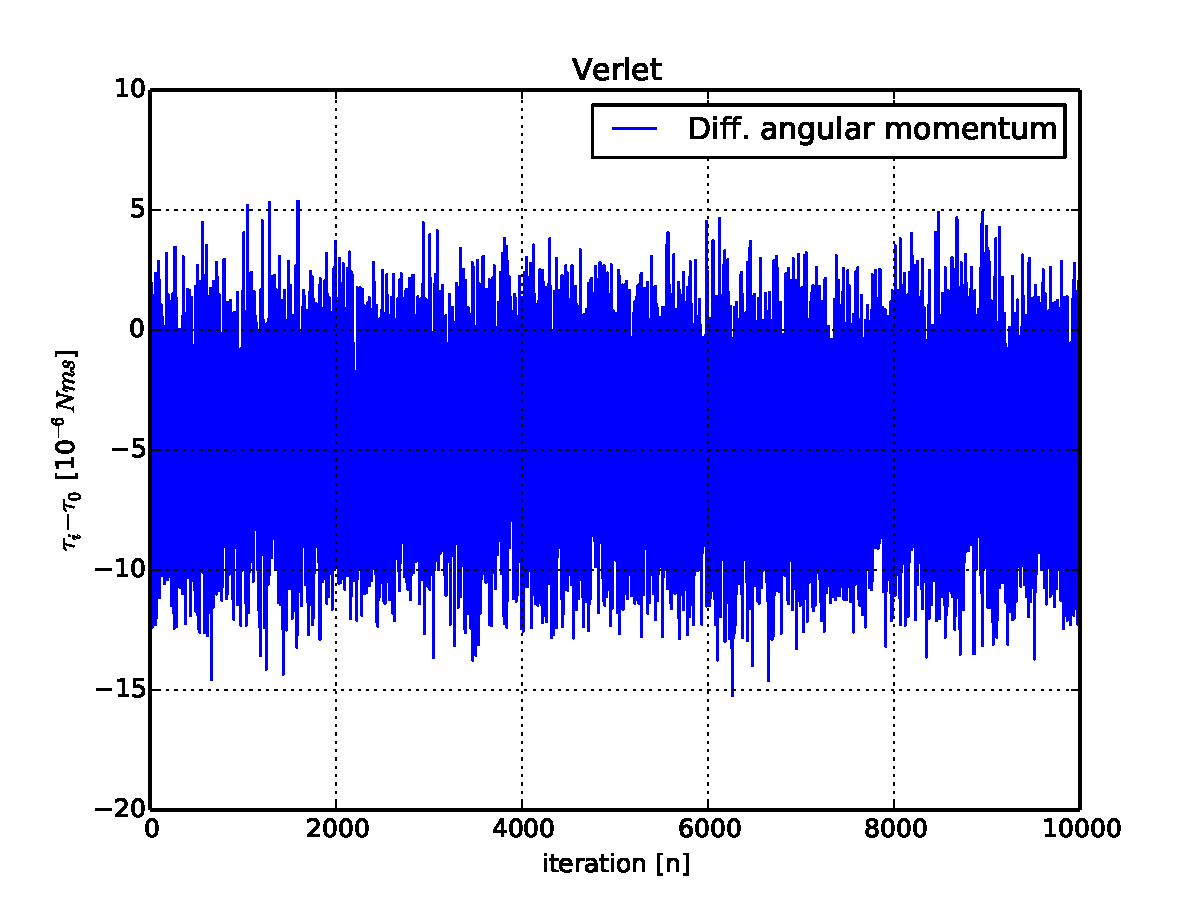
\includegraphics[width=\linewidth]{result/bilder/ang-momentum-verlet.pdf}
        \caption{}
    \end{subfigure}
    \caption{Both are figures are graphs of the angular momentum and how it differ from they intial value. a) is the Forward Euler method and b) is the Verlet-Velocity method. Forward Euler is once again not capable of conserving the value, but luckily for us the Verlet-Velocity method is. 
    }
    \label{fig:conserved-ang}
\end{figure}















\subsubsection{Escape velocity}

The assignment was to find the escape velocity for the earth by trial and error. Fortunate for us that we know some math and can calculate it. See section \ref{sec:escape-velocity} for this. But we started guessing \"randomly\" (winking Face emoji). Figure (\ref{fig:escape-velocity-low}) a) shows these guesses. Where we can see that the velocities around 8.8 au/year shots out and never returns. 
The algorithms only runs for 15 years and will thereby not see the 8.8 au/year return to orbit even tho it should. The plots were made by the data and python scripts in the directory \href{https://github.com/erikfsk/Project-3/tree/master/Project3/escape-velocity}{\textcolor{blue}{escape-velocity}}.

\begin{figure}[H]
    \centering
    \begin{subfigure}{0.5\textwidth}
        \centering
        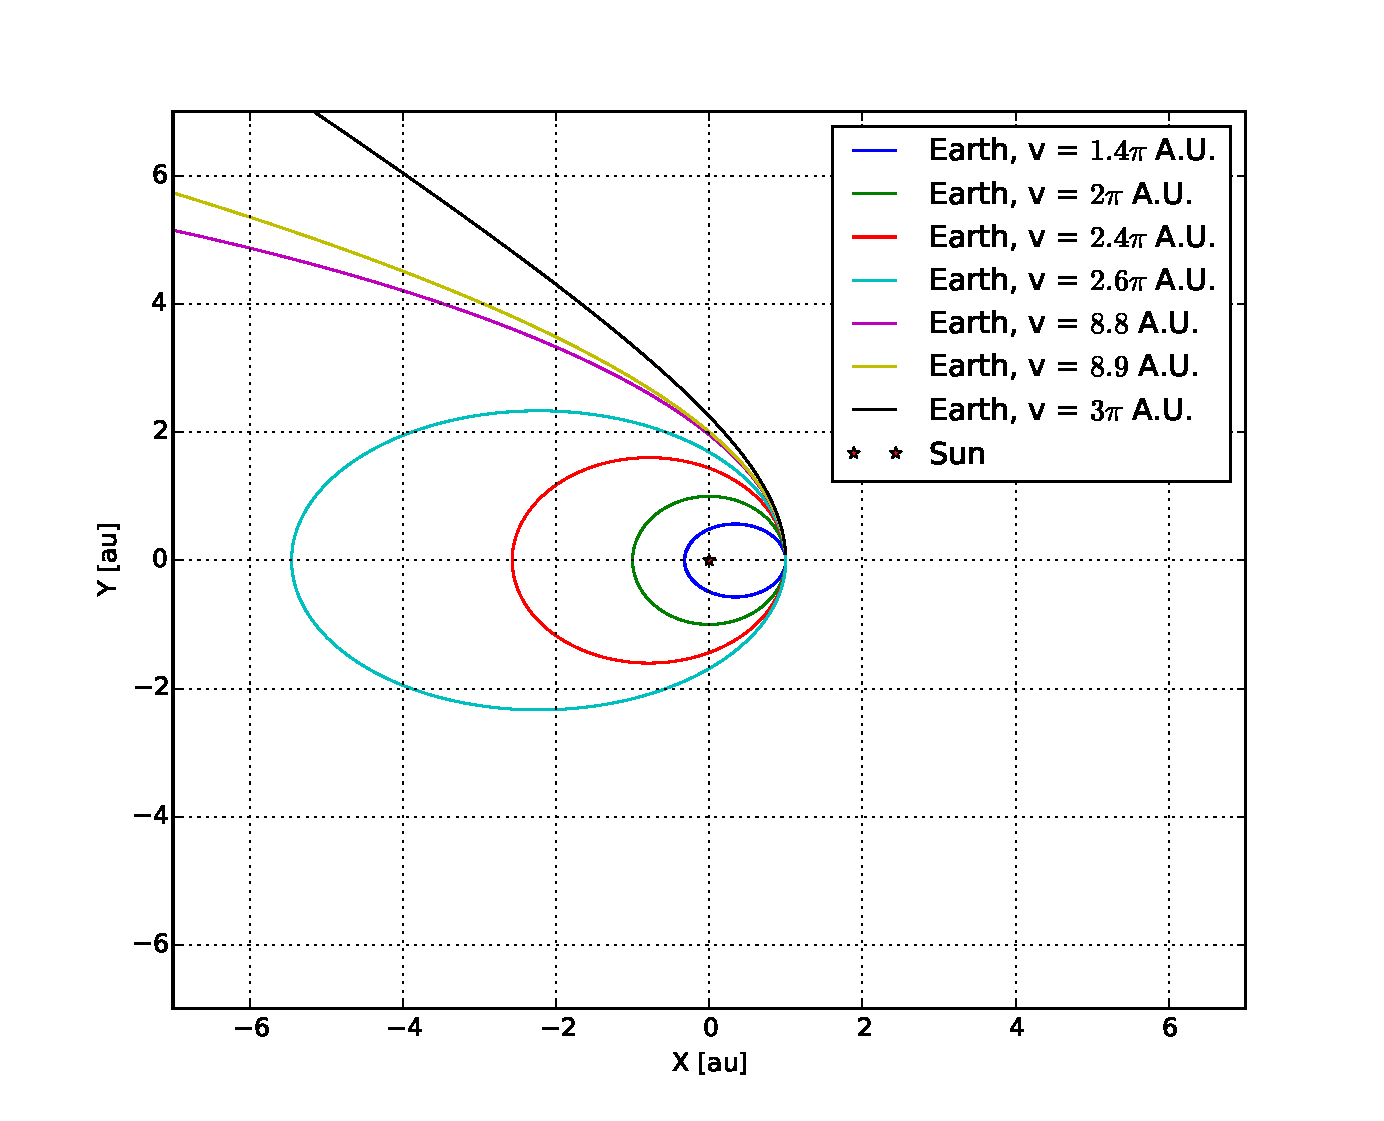
\includegraphics[width=\linewidth]{result/bilder/escape-velocity.pdf}
    	\caption{}
    \end{subfigure}%
    ~ 
    \begin{subfigure}{0.5\textwidth}
        \centering
        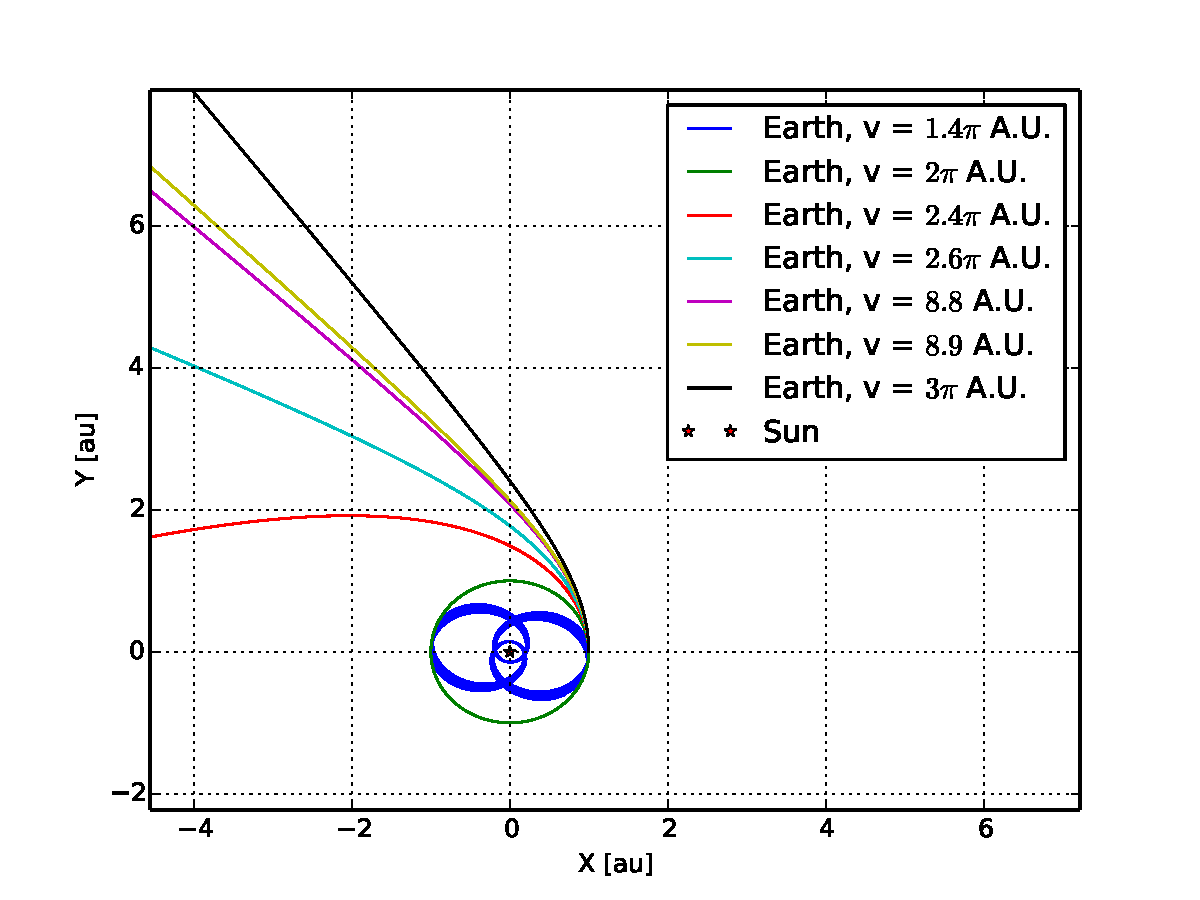
\includegraphics[width=\linewidth]{result/bilder/escape-velocity-r25.pdf}
        \caption{}
    \end{subfigure}
    \caption{a) Show how the orbits of earths with different initial velocity are. b) Shows the same as a) but this time the dependency of r in the denominator in equation (\ref{eq:newton}) is set to 3.5.}
    \label{fig:escape-velocity-low}
\end{figure}



\begin{figure}[H]
    \centering
    \begin{subfigure}{0.5\textwidth}
        \centering
        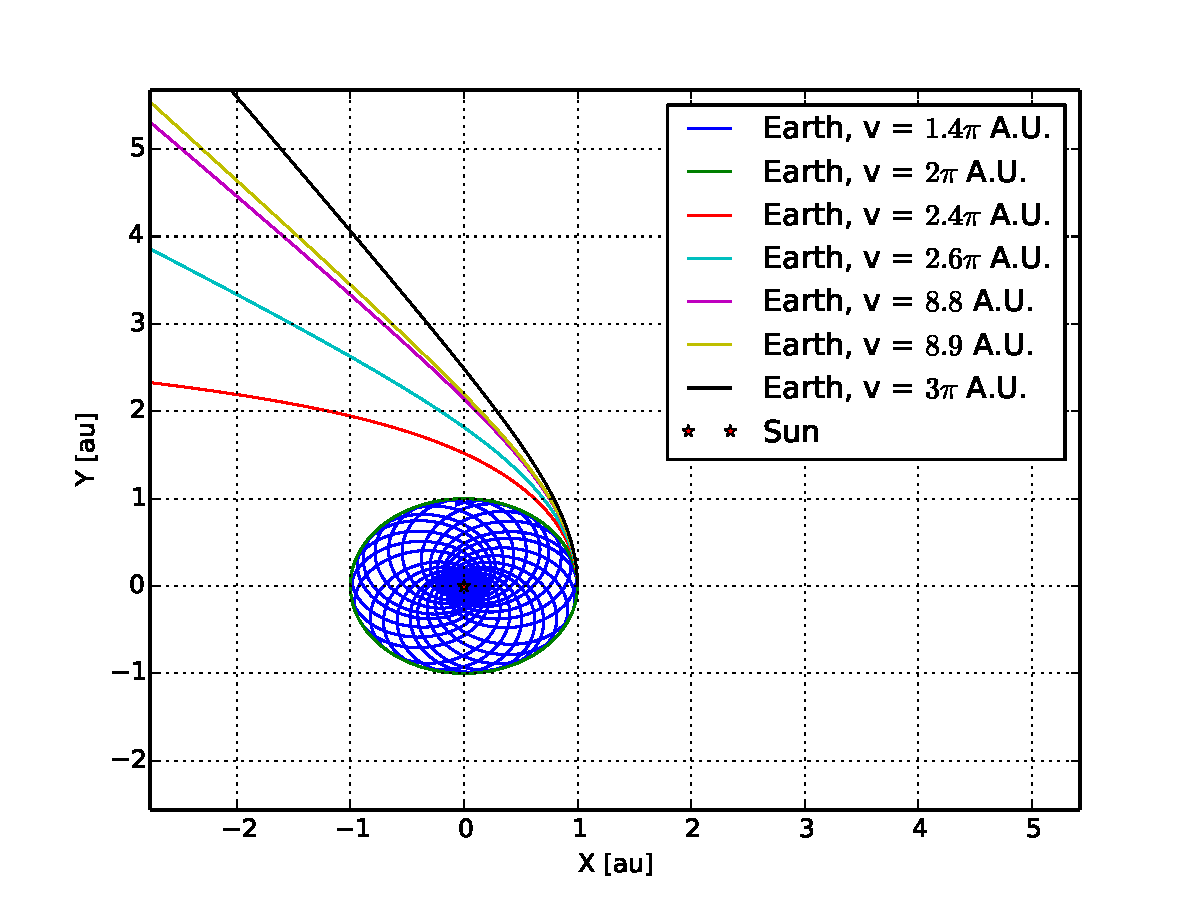
\includegraphics[width=\linewidth]{result/bilder/escape-velocity-r275.pdf}
    	\caption{}
    \end{subfigure}%
    ~ 
    \begin{subfigure}{0.5\textwidth}
        \centering
        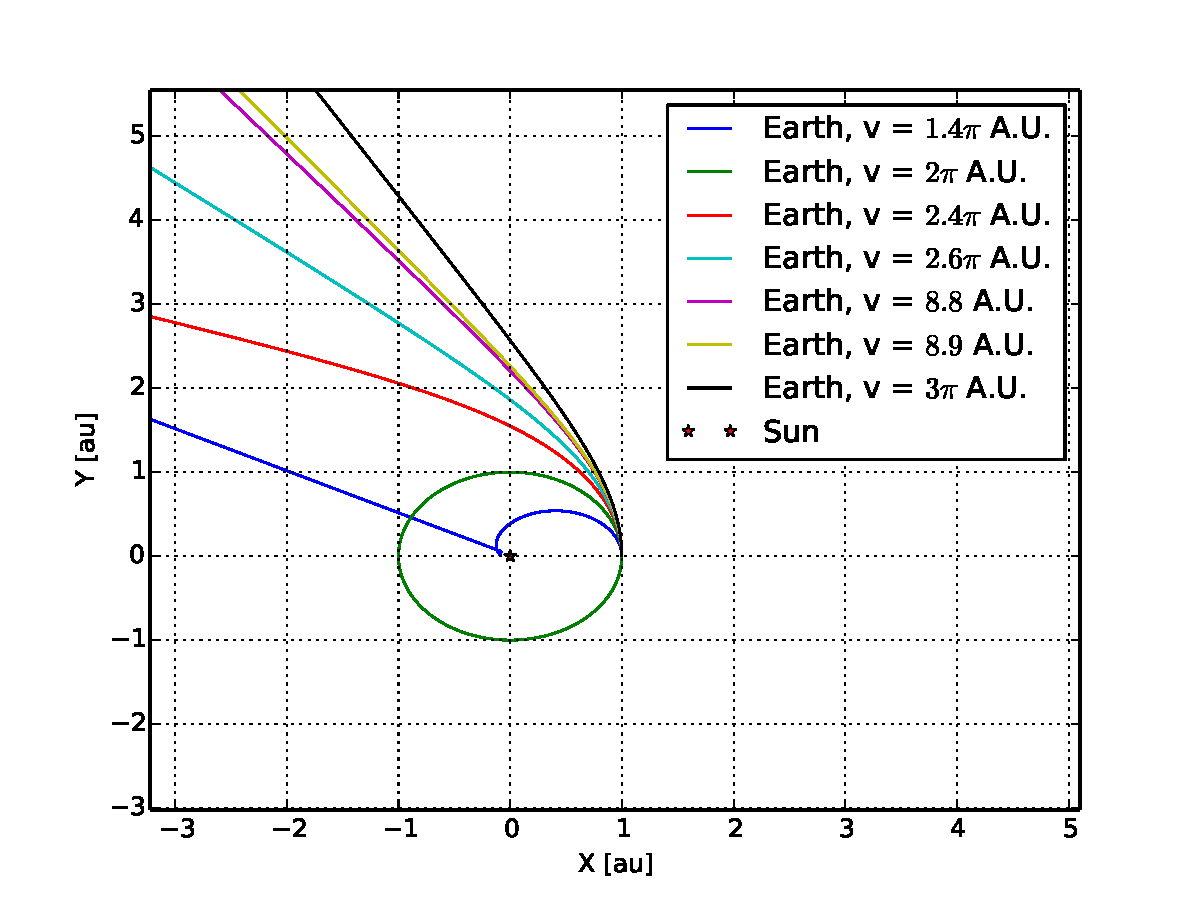
\includegraphics[width=\linewidth]{result/bilder/escape-velocity-r3.pdf}
        \caption{}
    \end{subfigure}
    \caption{a) Shows the same as figure (\ref{fig:escape-velocity-low}) but this time the dependency of r in the denominator in equation (\ref{eq:newton}) is set to 3.75. b) Shows the same as a) but this time the dependency of r in the denominator in equation (\ref{eq:newton}) is set to 4. }
    \label{fig:escape-velocity-high}
\end{figure}


Personally I feel extremly lucky for living in a universe with a r dependency of 2, but then again i probably would not exist if the dependency was different. All the other dependencies are very unstable for even the slightest change in velocity from a perfect circle.


















\subsection{Three body system}

\subsubsection{Fixed mass for jupitur}

\begin{figure}[H]
    \centering
    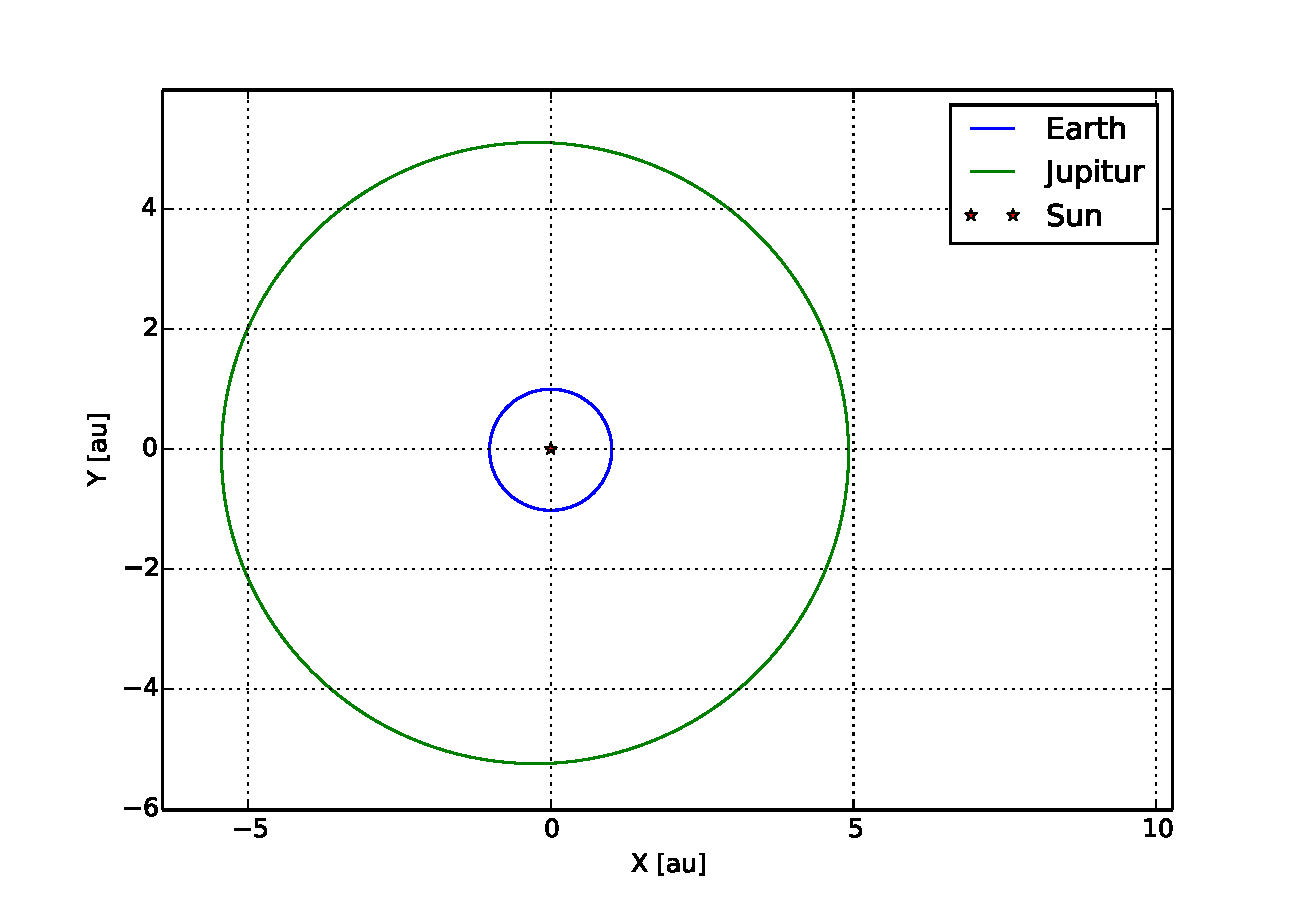
\includegraphics[width=\linewidth]{result/bilder/jupitur-mass.pdf}
    \caption{\href{https://github.com/erikfsk/Project-3/blob/master/Project3/3a/plot_earth_sun.py}{\textcolor{blue}{plot\_earth\_sun.py}}}
    \label{fig:three-body}
\end{figure}


\subsubsection{Varying mass for jupitur}

\begin{figure}[H]
    \centering
    \begin{subfigure}{0.5\textwidth}
        \centering
        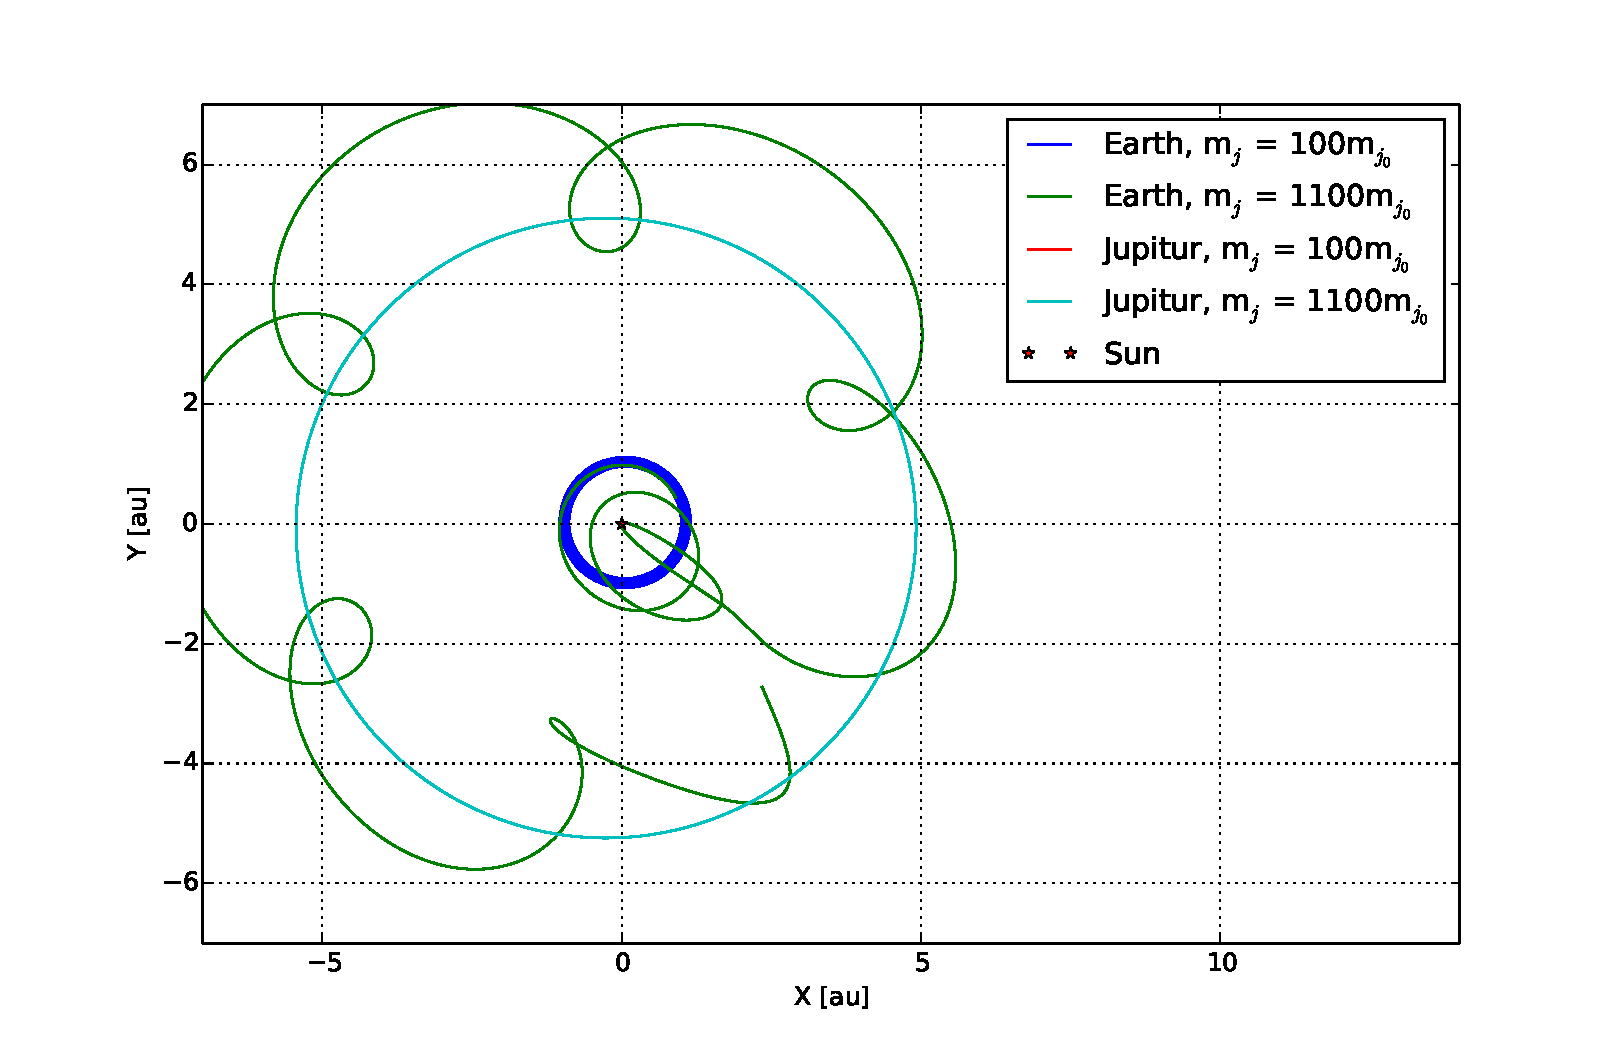
\includegraphics[width=\linewidth]{result/bilder/jupitur-mass-three.pdf}
    	\caption{}
    \end{subfigure}%
    ~ 
    \begin{subfigure}{0.5\textwidth}
        \centering
        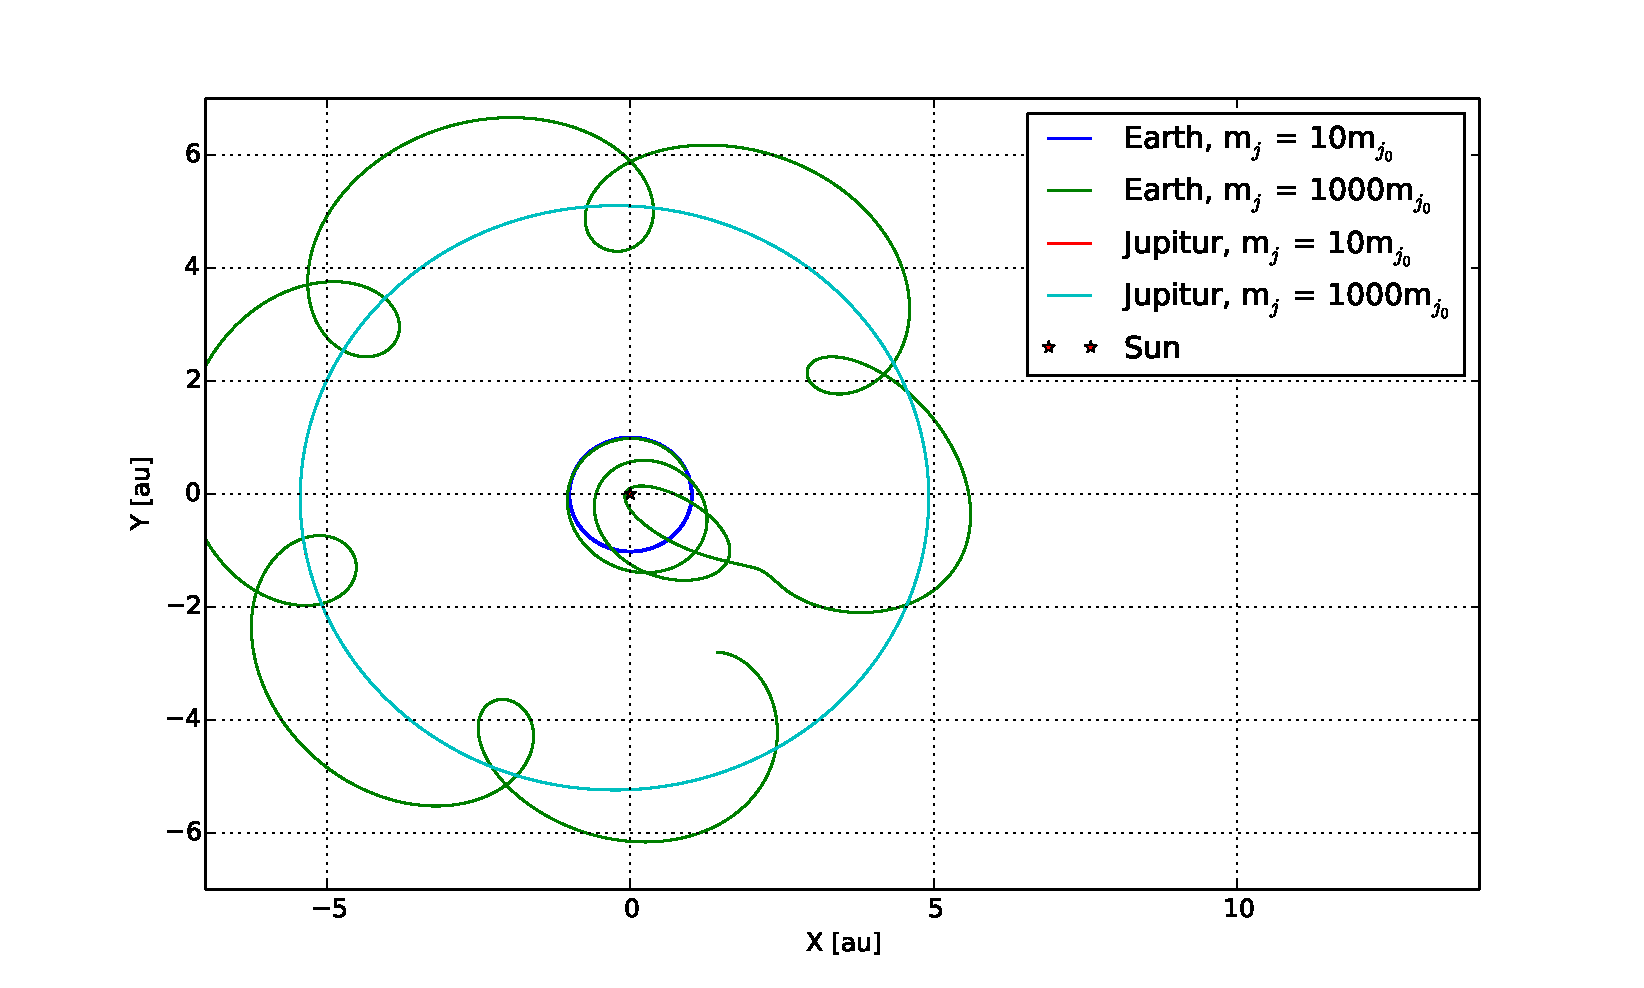
\includegraphics[width=\linewidth]{result/bilder/jupitur-mass-two.pdf}
        \caption{}
    \end{subfigure}
    \caption{\href{https://github.com/erikfsk/Project-3/blob/master/Project3/3a/plot_earth_sun.py}{\textcolor{blue}{plot\_earth\_sun.py}}}
    \label{fig:three-body-varying}
\end{figure}











\subsection{Solar system}


\subsubsection{Three planets and all moving}


\subsubsection{Solar system all moving}














\subsection{The perihelion precession of Mercury}

\subsubsection{missing this part}













